%KECReportFormat.tex
%%%%%%%%%%%%%%%%%%%%%%%%%%%%%%%%%%%%%%%%%%%%%%%%%%%%%%%%%%%%%%%%%%%%%%%%%%%
%DO NOT MAKE CHANGES IN THIS FILE

\documentclass[12pt, a4paper]{report}
\usepackage[left = 1.5in, right = 1in, top = 1in, bottom = 1in]{geometry}%for margin
\usepackage{amsfonts, amsmath, amssymb} %for mathematical equations
\usepackage{graphicx} %for images
\usepackage{times} %font Times New Roman Font
\usepackage{float} %required if you use H(strictly here) position for floats
\usepackage[skip = 8pt,tableposition=top, figureposition=bottom]{caption}%adjust spacing of captions and specify where captions are
\usepackage{hyperref} % for easy Navigation in document, also puts links in TOC, LOF, LOT...
\usepackage{setspace} %to change line spacing in some portion \singlespacing \onehalfspacing \doublespacing
\usepackage{acro} %for List of Abbrreviation and Symbol
\acsetup{first-style = short} % set to display only short form on the command \ac{}

%packages required for complex tables
\usepackage{bigstrut} 
\usepackage{multirow}

\renewcommand{\contentsname}{Table of Contents} %Change TOC Heading ... default is "Contents" 

\parindent 0pt	%removes the indent in paragraph
\setlength{\parskip}{18pt}	%for paragraph spacing
\renewcommand{\baselinestretch}{1.5}   %Line Spacing = 1.5 line-spaces

%to reduce spacing in sections
\usepackage{titlesec}
\titlespacing*{\section}{0pt}{0pt}{0pt} %left, top, bottom spacings
\titlespacing*{\subsection}{0pt}{0pt}{0pt}
\titlespacing*{\subsubsection}{0pt}{0pt}{0pt}
\titlespacing*{\paragraph}{0pt}{0pt}{0pt}
\titlespacing*{\subparagraph}{0pt}{0pt}{0pt}

%adjust fontsizes\ of sections
\titleformat*{\section}{\fontsize{14pt}{18pt}\bfseries}
\titleformat*{\subsection}{\fontsize{13pt}{18pt}\bfseries}
\titleformat*{\subsubsection}{\fontsize{12pt}{18pt}\bfseries}
\titleformat*{\paragraph}{\fontsize{12pt}{18pt}\bfseries}
\titleformat*{\subparagraph}{\fontsize{12pt}{18pt}\bfseries}

%to reduce separation between points in list
\usepackage{enumitem}
\setlist[enumerate]{nosep} % no separation between items in enumerate
\setlist[itemize]{nosep} % no separation between items in itemize
%use \vspace{-18pt} before list to reduce paragraph spacing between list and preceeding paragraph.

%Changes for Chapter Heading Spacing and formats for numbered chapters
\makeatletter
\def\@makechapterhead#1{%
  %\vspace*{50pt}%
  {  \MakeUppercase{\ifnum \c@secnumdepth >\m@ne
        \fontsize{16pt}{1}\bfseries \@chapapp \space \thechapter\vspace{5pt}\\
    \fi
    \interlinepenalty\@M
     \bfseries #1}\par\nobreak
    %\vskip 0pt
  }}
\makeatother

%%%%%%%%%%%%%%%%%%%%%%%%%%%%%%%%%%%%%%%%%%%%%%%%%%%%%%%%%%%
%to adjust Heading spacings and fonts For unnumbered chapters, TOC, LOF ...
\makeatletter
% Redefine the \chapter* header macro to remove vertical space
\def\@makeschapterhead#1{%
  %\vspace*{50\p@}% Remove the vertical space
  {\newpage \parindent \z@ \raggedright
    \normalfont
    \interlinepenalty\@M
    \center \fontsize{16pt}{1} \bfseries \MakeUppercase{#1}\par\nobreak
    %\vskip 18\p@ % adjust space after heading 18pt
  }}
\makeatother 
%%%%%%%%%%%%%%%%%%%%%%%%%%%%%%%%%%%%%%%%%%%%%%%%%%%%%%%%%%%

%%%%%%%%%%%%%%%%%%%%%%%%%%%%%%%%%%%%%%%%%%%%%%%%%%%%%%%%%%%%%%%%%%%%%%%%%%%
% newcommand for generating Cover Page
\newcommand{\KECcoverpage}
{
\begin{titlepage}
\begin{center}
\Large{\textbf{KANTIPUR ENGINEERING COLLEGE}}\\
\large{\textbf{(Affiliated to Tribhuvan University)}}\\
\large{\textbf{Dhapakhel, Lalitpur}}\\
\vfill	%vertically fill the space 
\begin{figure}[h] % h: put logo "here"
\begin{center}
\includegraphics[width=25mm, height = 25mm]{images/logo.png}
\end{center}
\end{figure}

\large{\textbf{[Subject Code: \subCode]}}\\ %Change This Line
\large{\textbf{A \MakeUppercase{\project} \MakeUppercase{\doc} ON}}\\ %Change This Line
\Large{\textbf{\MakeUppercase{\projectTitle}}}\\

\vfill	%vertically fill the space 
\large{\textbf{Submitted by:}}\\
\large{\textbf{\submittedBy}}\\
\vfill	%vertically fill the space 
\textbf{A \MakeUppercase{\project} SUBMITTED IN PARTIAL FULFILLMENT OF THE REQUIREMENT FOR THE DEGREE OF \MakeUppercase{\degree}}\\

\vfill	%vertically fill the space 
\large{\textbf{Submitted to:}}\\
\large{\textbf{\submittedTo}}\\
\vfill
\large{\textbf{\defMonth, \defYear}}
\pagebreak
\end{center}
\end{titlepage}
}
%%%%%%%%%%%%%%%%%%%%%%%%%%%%%%%%%%%%%%%%%%%%%%%%%%%%%%%%%%%%%%%%%%%%%%%
% newcommand for generating Cover Page
%Title Page
\newcommand{\KECtitlepage}
{
\begin{titlepage}
\begin{center}
\Large{\textbf{\MakeUppercase{\projectTitle}}}\\

\vfill	%vertically fill the space 

\large{\textbf{Submitted by:}}\\
\large{\textbf{\submittedBy}}\\


\ifhassupervisor % Displays Supervisor name only if \hassupervisortrue
	\vfill	%vertically fill the space 
	\large{\textbf{Supervised by:}}\\
	\large{\textbf{\supervisor}}\\
	\large{\textbf{\degSup}}\\
\fi

\vfill	%vertically fill the space 
\textbf{A \MakeUppercase{\project} SUBMITTED IN PARTIAL FULFILLMENT OF THE REQUIREMENT FOR THE DEGREE OF \MakeUppercase{\degree}}\\

\vfill	%vertically fill the space 
\large{\textbf{Submitted to:}}\\
\large{\textbf{\submittedTo}}\\
\large{\textbf{Kantipur Engineering College}}\\
\large{\textbf{Dhapakhel, Lalitpur}}\\

\vfill
\large{\textbf{\defMonth, \defYear}}
\thispagestyle{empty}\\ %to remove page number
\pagebreak
\end{center}
\end{titlepage}
}
%%%%%%%%%%%%%%%%%%%%%%%%%%%%%%%%%%%%%%%%%%%%%%%%%%%%%%%%%%%%%%%%%%%%%%
%command for copyright page
\newcommand{\KECcopyright}
{
\chapter*{Copyright}%Required only for Final Defense of Major Project
\addcontentsline{toc}{chapter}{Copyright}
The author has agreed that the library, Kantipur Engineering Collage, may make this report freely available for inspection. Moreover the author has agreed that permission for extensive copying of this report for scholarly purpose may be granted by the supervisor(s), who supervised the project work recorded herein or, in their absence, by the Head of the Department wherein this project was done. It is understood that due recognition will be given to the author of this report and to the \submittedTo, Kantipur Engineering College in any use of the material of this report. Copying or publication or other use of this report for financial gain without approval of the \submittedTo, Kantipur Engineering College and author’s written permission is prohibited.\par Request for permission to copy or to make any other use of the material in this report in whole or in part should be addressed to:

Head\\
\submittedTo\\
Kantipur Engineering College\\
Dhapakhel, Lalitpur\\
Nepal
}
%%%%%%%%%%%%%%%%%%%%%%%%%%%%%%%%%%%%%%%%%%%%%%%%%%%%%%%%%%%%%%%%%%%%%%
%command for Approval Letter
\newcommand{\KECapproval}
{
\chapter*{Kantipur Engineering College
\vskip -10pt}%Required only for Final Defense of Major Project
\begin{center}
\fontsize{12.8pt}{1} %size decreaced to adjust department name in single line
\textbf{
\MakeUppercase{\submittedTo}\\ %for department name
}
\vskip 10pt
\fontsize{16pt}{1}
\textbf{APPROVAL LETTER}
\end{center}
\vskip -16pt
\addcontentsline{toc}{chapter}{Approval Letter}%
The undersigned certify that they have read and recommended to the Institute of Engineering for acceptance, a project report entitled "\projectTitle " submitted by \\
\submittedBy \\
in partial fulfillment for the degree of \degree. \par
{\vspace{25pt}
..........................................\\
Supervisor\\
\supervisor \\
\degSup\\
\vspace{25pt}\\
..........................................\\
External Examiner\\
\external\\
\degExternal\\
\vspace{25pt}\\
..........................................\\
\hod\\
Head of Department\\
\submittedTo
\vspace{10pt}\\
Date: \defMonth\space\defDay ,\space \defYear
\singlespacing\par
} %single spacing for the texts inside {}
}

%command for list of abbreviations
\newcommand{\KECloa}
{
\chapter*{List of Abbreviations}
\addcontentsline{toc}{chapter}{List of Abbreviations}
\vskip -42pt % to reduce space due to invisivle acronym class name
{
\singlespacing
\printacronyms[include-classes=abbr, name= ]
}

}

%command for list of symbols
\newcommand{\KEClos}
{
\chapter*{List of Symbols}
\addcontentsline{toc}{chapter}{List of Symbols}
\vskip -42pt % to reduce space due to invisivle acronym class name{
{
\singlespacing
\printacronyms[include-classes=symbol, name= ]
}
}

%command to adjust toc, lof, lot spacing
\newcommand{\KECadjusttocspacings}
{
\parskip 0pt % to remove paragraph spacing in TOC, LOF ...
\renewcommand{\baselinestretch}{0.1} % to adjust line spacing in toc
\newcommand*{\noaddvspace}{\renewcommand*{\addvspace}[1]{}}
\addtocontents{lof}{\protect\noaddvspace} %remove extra vertical space in LOF
\addtocontents{lot}{\protect\noaddvspace} %remove extra vertical space in LOT
} %includes the file KecReportFormat.tex that include all necessary formattings
%%%%%%%%%%%%%%%%%%%%%%%%%%%%%%%%%%%%%%%%%%%%%%%%%%%%%%%%%%%%%%%%%%%%%%%%%%%
%Define Macros for Details of your Project
\newcommand{\project}{Minor Project} %Specify "Major Project" or "Minor Project"
\newcommand{\projectTitle}{House Price Prediction System Using Multiple Linear Regression} %specify "Title" of Your Project
\newcommand{\doc}{Final Report} % specify the document you are preparing eg. "Proposal", "Mid-Term Report" or "Final Report" 
% Note that You have to sibmit "Final Report" for Pre-final defense as well.
\newcommand{\subCode}{CT654} %specify Subject of Your Project
\newcommand{\degree}{Bachelor in Computer Engineering} %specify your degree
\newcommand{\submittedBy}%Specify Names and Roll/Symbol Numbers of the Project Group Members
{
%Edit Member Names and Roll/Symbol No. and adjust width (\makebox[width]) if necessary 
\makebox[6cm]{Aman Devkota  \hfill[KAN076BCT010]}\\
\makebox[6cm]{Ankur Karmacharya  \hfill[KAN076BCT013]}\\
\makebox[6cm]{Prashad Adhikary  \hfill[KAN076BCT056]}
%\makebox[9cm]{Member Name \hfill [Roll/Symbol No.]}\\
} % Note that You must write your "Symbol Numbers"(Exam Roll Numbers) for Final Defenses

\newcommand{\submittedTo}{Department of Computer and Electronics Engineering} %specify your department
\newcommand{\hod}{Er. Rabindra Khati} %specify Head ot the department
\newcommand{\defYear}{2023} %Defense Year
\newcommand{\defMonth}{March} %Defense Month- January, February, ...
\newcommand{\defDay}{26} %specify Defense Day- 1, 2, ...

\newif\ifhassupervisor
\hassupervisorfalse % to display supervisor name use command- \hassupervisortrue
\newcommand{\supervisor}{none} % Specify Name of Supervisor for Major Project (write "none" if no Supervisor is assigned)
\newcommand{\degSup}{Supervisor's Designation\\Second Line of Designation (if required)} %Specify Designation of Supervisor for Major Project, use multiple lines (\\) if necessary
\newcommand{\external}{External's Name} %Specify Name of External for Major Project (Required for Black Book)
\newcommand{\degExternal}{External's Designation\\Second Line of Designation (if required)} %Specify Name of External for Major Project (Required for Black Book) , use multiple lines (\\) if necessary
%%%%%%%%%%%%%%%%%%%%%%%%%%%%%%%%%%%%%%%%%%%%%%%%%%%%%%%%%%%%%%%%%%%%%%%%%%%

%%%%%%%%%%%%%%%%%%%%%%%%%%%%%%%%%%%%%%%%%%%%%%%%%%%%%%%%%%%%%%%%%%%%%%%%%%%

%%%%%%%%%%%%%%%%%%%%%%%%%%%%%%%%%%%%%%%%%%%%%%%%%%%%%%%%%%%%%%%%%%%%%%%%%%%%%%%%%%%%%%%%%%%%%%%%%%%%

%%%%%%%%%%%%%%%%%%%%%%%%%%%%%%%%%%%%%%%%%%%%%%%%%%%%%%%%%%%%%%%%%%%%%%%%%%
%The Document
\begin{document}
\KECcoverpage  % command defined in KECReportFormat
\KECtitlepage  % command defined in KECReportFormat

\pagenumbering{roman} % starts pagenumberins in Roman numerals i, ii, ...

%Copyright Page is required for FINAL REPORT only. Comment this section for other Reports.
%\KECcopyright % defined in KECReportFormat.tex

%Approval Page is required for FINAL(Black Book Binded) REPORT of MAJOR PROJECT only. Comment this section for other Reports. 
%\KECapproval % defined in KECReportFormat.tex

\chapter*{Abstract} % The summary of your report
\addcontentsline{toc}{chapter}{Abstract}%to include this chapter in TOC 
The growth of Machine learning has been rapid in this past decade. Many applications evolve in Machine learning day by day. One such application is the house price prediction. Humans are very thoughtful when they want to make investments in a house. The prices for houses have been changing every year that has necessitated the modelling of a house price prediction system. This system will make use of the features of the house such as number of bathrooms available, total area, location of the house etc. to generate an estimated price for the house with the help of multiple linear regression.
\par
\textbf{\textit{Keywords$-$}} \emph{multiple linear regression, house price prediction system}

\chapter*{Acknowledgment}
\addcontentsline{toc}{chapter}{Acknowledgment}%to include this chapter in TOC
We would like to express sincere gratitude to Department head Er. Rabindra Khati, Project Co-ordinator Er. Bishal Thapa and all the faculty members of Kantipur Engineering College for the continuous support during this project for their patience, motivation,enthusiasm, and immense knowledge. Their guidance helped us in all time of research, development and implementation of this project.   \par
%Finally we would like to thank our family and friends for all the support and encouragement.\par
%to display members name under Acknowledgement
\begin{flushright}
\vskip -20pt
\setstretch{1.2}
\submittedBy

\end{flushright}

%to adjust spacings for TOC, LOF, LOT
{
%%%%%%%%%%%%%%%%%%%%%%%%%%%%%%%%%%%%%%%%%%%%%%%%%%%%%%%%%%%%%%%%%%%%%%%%%%%
%TOC, LOF and LOT
\KECadjusttocspacings % defined in KECReportFormat.tex to adjust spacings
\makeatletter
% to add vskip of 18 point which is reduced when parskip is set to 0 in \LECadjustspacings
\def\@makeschapterhead#1{%
  %\vspace*{50\p@}% Remove the vertical space
  {\newpage \parindent \z@ \raggedright
    \normalfont
    \interlinepenalty\@M
    \center \fontsize{16pt}{1} \bfseries \MakeUppercase{#1}\par\nobreak
   % \vskip 18\p@ % adjust space after heading 18pt
  }}
\makeatother 

\tableofcontents % prints table of contents
\listoffigures % prints list of figures
\addcontentsline{toc}{chapter}{List of Figures}
%\listoftables % prints list of table
%\addcontentsline{toc}{chapter}{List of Tables}
}
%%%%%%%%%%%%%%%%%%%%%%%%%%%%%%%%%%%%%%%%%%%%%%%%%%%%%%%%%%%%%%%%%%%%%%%%%%%

%comment this chapter if you don't have List of Abbreviations
%\KECloa % defined in KECReportFormat

%comment this chapter if you don't have List of Symbols
%\KEClos % defined in KECReportFormat

\newpage
\pagenumbering{arabic} % starts pagenumbering in arabic numerals

\chapter{Introduction}
\section{Background}\label{sec:bkgrnd}%label your section if you require to refer them somewhere else in your document.
Usually when people want to buy a house, they look for a house which has a reasonable cost, and which has all the desired features they want in the house. The house price prediction will help them to decide whether the house they desire to buy is worth of the price or not. Similar is the case with people who want to sell the house. By making use of the house price prediction system, the seller would be able to decide what all features he/she could add in the house so that the house can be sold for a higher price. \cite{kaushal2021house}
\par
Modelling uses machine learning algorithms, where machine learns from the data and uses them to predict a new data. The most frequently used model for predictive analysis is regression. As we know, the proposed model for accurately predicting future outcomes has applications in economics, business, banking sector, health care industry, e-commerce, entertainment, sports etc. One such method used to forecast house prices are based on multiple factors. In metropolitan cities, the prospective home buyer considers several factors such as location, size of the land, road conditions, parking availability and most importantly the house price. Multiple linear regression is one of the statistical techniques for assessing the relationship between the (dependent) target variable and several independent variables. Regression techniques are widely used to build a model based on several factors to predict price. \cite{manasa2020machine}
 \par
Multiple linear regression is a statistical technique that can be used to analyze the relationship between a single dependent variable and several independent variables. The objective of multiple linear regression analysis is to use the independent variables whose values are known to predict the value of the single dependent value.
\par
The dataset that we are using contains the data about houses in Bangalore from the year 2019. It contains the following attributes:\\
Area: Area of the property in square feet\\
BHK: Number of bedrooms along with 1 hall and 1 kitchen\\
Bathrooms: Number of bathrooms\\
Location: Location in which property lies\\
Price: This is the Price of property in INR\\
Area Type: It’s an Apartment or Builder Floor

\section{Problem Definition}
%\vspace{-18pt}
Prices of real estate properties are sophisticatedly linked with our economy. Despite this, we do not have accurate measures of housing prices based on the vast amount of data available. Therefore, the goal of this project is to use machine learning to predict the selling prices of houses based on many factors.
\section{Objectives}
The primary objectives of this projects are as follows:
\vspace{-18pt}
\begin{enumerate}[label=\roman*.]
\item To predict house prices on the basis of various parameters.
\end{enumerate}

\section{Project Features}
The project will be able to accomplish following:
\vspace{-18pt}
\begin{itemize}
\item Low cost
\item Accurate
\item User friendly 
\end{itemize}

\section{Application Scope}
The application scope of our project is in real estate business. Our project will allow the buyer to get an idea of what amount of money he/she has to spend in order to buy the desired house. It will also allow the seller to get information regarding what the estimated worth of house is and how he/she can maximize the profit gained by selling the house.

\section{System Requirement}
\vspace{-18pt}
\subsection{Software Requirements}
\vspace{-10pt}
\begin{enumerate}
\item[] Windows/Linux/Mac
\item[] HTML/CSS/JS
\item[] Jupyter Notebook
\item[] Python IDE
\end{enumerate}
\subsection{Hardware Requirements}
\vspace{-10pt}
\begin{enumerate}
\item[] PC with at least 4-8 GB RAM
\item[] Higher graphics of at least 2 GB
\end{enumerate}
\label{tblSampleTable}
%\end{table}

\section{Project Feasibility}
\vspace{-18pt}
\subsection{Technical Feasibility}
\vspace{-18pt}
The technical feasibility assessment is focused on gaining in understanding of the present technical resources required by the system and their applicability to the expected needs of the proposed system. Regarding the proposed system, the technical requirement includes a PC.
\vspace{-18pt}
\subsection{Operational Feasibility}
\vspace{-18pt}
The user will not need any formal knowledge about programming so our project is operationally feasible.
\vspace{-18pt}
\subsection{Economic Feasibility}
\vspace{-18pt}
The purpose of the economic feasibility assessment is to determine the positive economic benefits to the user that the proposed system will provide. Most of the software used for the development is free. Thus, the project is economically feasible.
\vspace{-18pt}
\subsection{Schedule Feasibility}
\vspace{-18pt}
\begin{figure}[!h] % tbh means top, bottom or here (priority: left to right)
\begin{center}
	%\includegraphics[width = 3in]{images/logo.png}
	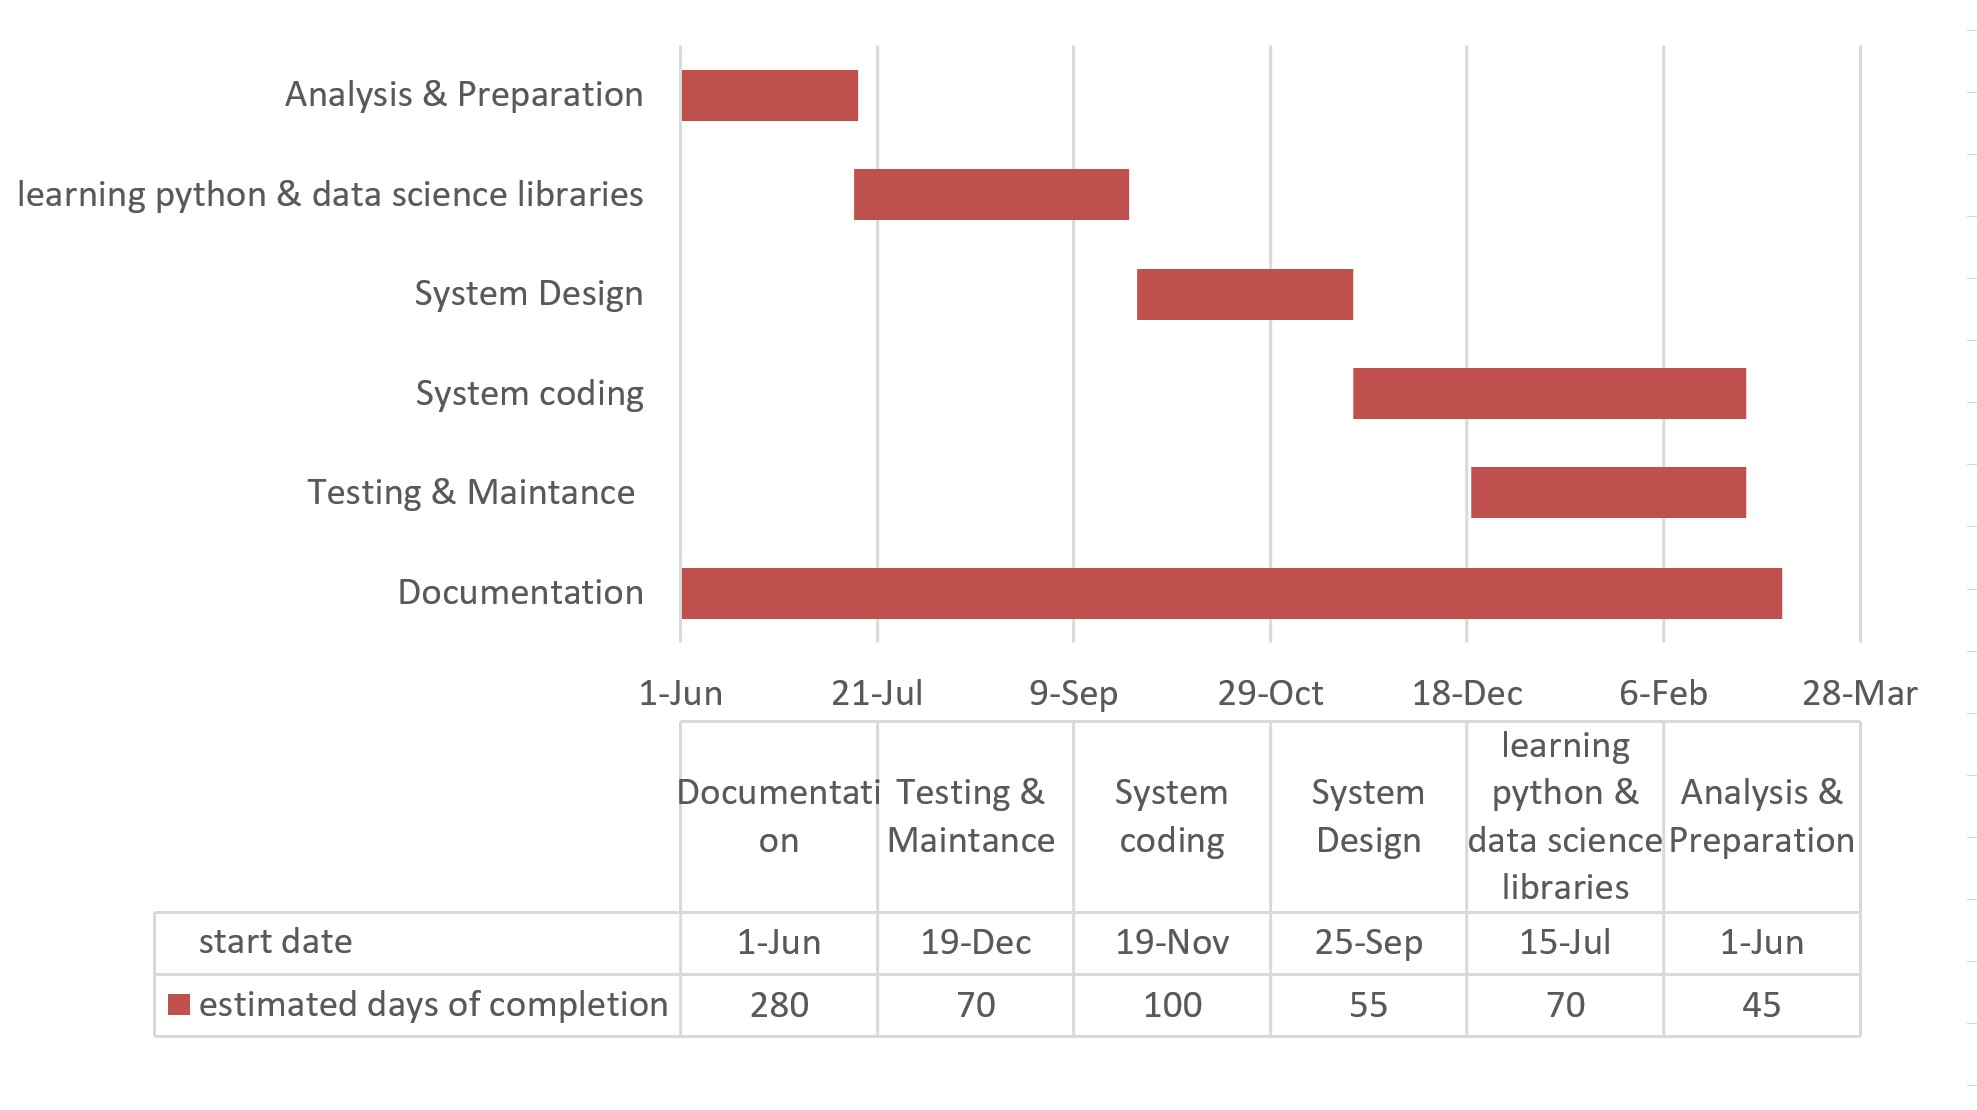
\includegraphics[width=6in]{Screenshot 2023-03-23 005901.jpg} 
	\caption{Gantt Chart} %figure name
	\label{figGanttChart} % for referencing
\end{center}
\end{figure}
\chapter{Literature Review}
\vspace{-18pt}
\section{Related Projects}
\vspace{-18pt}
\subsection{Zillow}
\vspace{-18pt}
 Zillow is a popular online real estate marketplace that provides an automated valuation model called the Zestimate. This model uses a combination of data from public records, user-submitted data, and machine learning algorithms to predict the value of a home.
 \vspace{-10pt}
\subsection{Redfin's Home Value Estimator}
\vspace{-18pt}
Redfin is another online real estate marketplace that provides a home value estimator tool that uses machine learning algorithms to predict the value of a home based on its location, features, and recent sales in the area.
\vspace{-10pt}
\subsection{House Canary}
\vspace{-18pt}
HouseCanary is a real estate analytics company that provides a range of services, including home value estimates and forecasts, neighborhood insights, and market analytics. Their home value estimates are based on a proprietary machine learning model that analyzes millions of data points.
\vspace{-10pt}
\subsection{Propmix.io}
\vspace{-18pt}
PropMix.io is a real estate data and analytics platform that offers a range of tools for real estate professionals, including a home value estimator that uses machine learning algorithms to predict the value of a home based on its features and location.
\vspace{-10pt}
\section{Related Works}
Anirudh Kaushal and Achyut Shankar researched in detail about house price prediction using multiple linear regression method. In the paper “House Price Prediction Using Multiple Linear Regression” published on April 25, 2021 there is explanation about filtering of data set, data processing, training and evaluating multiple linear regression model. \cite{kaushal2021house} Manasa, J., Gupta, R., \& Narahari, N. S. studied and compared the algorithms for estimation of price of houses in city of Bengaluru in the paper “Machine learning based predicting house prices using regression techniques”. \cite{manasa2020machine} M. Thamarai, S P. Malarvizhi have compared the decision tree and regression algorithms in the paper “House Price Prediction Modeling Using Machine Learning”. The basis of comparison was accuracy, MAE, MSE and RMSE. \cite{thamarai2020house} Rana, V. S., Mondal, J., Sharma, A., \& Kashyap, I. have studied in detail about the machine learning algorithms and compared the results obtained by each to learn about the algorithm most suitable to use in the house price prediction system in their paper “House Price Prediction Using Optimal Regression Techniques”.\cite{Rana2020HousePP} Madhuri, C. R., Anuradha, G., \& Pujitha, M. V. studied on different regression algorithms. In the paper “House price prediction using regression techniques: a comparative study” published on March, 2019, there is explanation about different types of regression methods and their accuracy to predict the values. \cite{madhuri2019house}
\chapter{Methodology}
  \section{Working Mechanism}
The development of house price prediction system involves major steps which is 
depicted in the diagram given below:
\begin{figure}[tbh] % tbh means top, bottom or here (priority: left to right)
\begin{center}
	%\includegraphics[width = 3in]{images/logo.png}
	%\includegraphics[width = 4in]{images/q.jpg}
	%\caption{} %figure name
	%\label{figObjectDetectionusingYOLO} % for referencing
\end{center}
\end{figure}
\subsection{Load the data set}
The raw data of different houses with different parameters as independent values and the price of the house as dependent value are collected and are loaded for data analysis.
\subsection{Add dummy variables}
The parameters in the data set like addresses are string values but the multiple linear regression can only accept numerical values so they are need to be converted into numerical values. In order to convert it we need to give them the value 0 and 1 on the basis that they are available but there may arise dummy trap problem (when two independent parameters affect each other which can cause conflict in multiple linear regression). So to solve this problem the dummy variables should be one less than the n number of string valued parameters.
\subsection{Filter the dataset}
All the parameters in the raw data set are not needed for multiple linear regression as some of the parameters have little or no significance in changing the price of the house. So to filter out the useless parameters, we find the single correlation between price of the house and the parameters. Correlation coefficients are used to measure the strength of the linear relationship between two variables. A correlation coefficient greater than zero indicates a positive relationship while a value less than zero signifies a negative relationship.If the correlation is very low or near to zero, they can be neglected.\\
Mathematical calculation for correlation
\begin{equation}
(r_{xy}) =\frac {(n\sum{xy}-\sum{x}\sum{y})}{(\sqrt{[n\sum{x^2}-(\sum{x})^2][n\sum{y^2}-(\sum{y})^2]}}
\end{equation}
We used Regular expression to filter out the location attributes.
\subsection{Split the data set into train set and test set}
The data set is divided in train set and test set so that the train set can be used for training the model.
\subsection{Statistical Calculations}
For the multiple linear regression, we need to find the values for $\sum{x},\sum{xy},...\sum{x_{n}}$ etc. which are calculated in this stage.
\subsection{Representing the normal equation of multiple linear regression in matrix form}
The equation of plane is
\begin{equation}
x=w_{0}+w_{1}x_{1}+w_{2}x_{2}+.....w_{N}x_{N}
\end{equation}
Here,$ x_{1},x_{2},....x_{N}$ are independent parameter variables and x is dependent parameter variable. The intercept is $w_{0}$ and coefficients are $w_{1},w_{2},....w_{N}$.\\
Now to find the values of $w_{0},w_{1},w_{2},...w_{N}$, we need the normal equations which are as follows:
\begin{eqnarray}
\sum{x}= nw_{0}+w_{1}\sum{x_{1}}+w_{2}\sum{x_{2}}+.....w_{N}\sum{x_{N}}\\
\sum{x x_{1}}= w_{0}\sum{x_{1}}+w_{1}\sum{x_{1}}^2+w_{2}\sum{x_{1}x_{2}}+.....w_{N}\sum{x_{1}x_{N}}\\
\sum{x x_{2}}= w_{0}\sum{x_{2}}+w_{1}\sum{x_{1}x_{2}}+w_{2}\sum{x_{2}}^2+.....w_{N}\sum{x_{2}x_{N}}
\end{eqnarray}
\begin{center}
:
\end{center}
\begin{equation}
\sum{x x_{N}}= w_{0}\sum{x_{N}}+w_{1}\sum{x_{1}x_{N}}+w_{2}\sum{x_{2}x_{N}}+.....w_{N}\sum{x_{N}}^2
\end{equation}
Python does not recognize equations so we need to represent these equations in matrix form for further calculations.
\subsection{ Calculation of intercept and coefficients using Gauss Elimination}
To find the values of $w_{0},w_{1},w_{2},...w_{N}$, we need to solve the matrices. For this we use the Gauss Elimination method.\\
Algorithm:
\vspace{-18pt}
\begin{enumerate}
\item Start
\item Declare the variables and read the order of the matrix N
\item Take the coefficients of the linear equations as:\\
Do for k= 1 to n\\
Do for j = 1 to n+1\\
Read a[k][j]\\
End for j\\
End for k
\item Do for k= 1 to n-1\\
Do for i= k+1 to n\\
Do for j= k+1 to n+1\\
a[i][j] = a[i][j] -a[i][k]/a[k][k]*a[k][j]\\
End for j\\
End for i\\
End for k
\item Compute x[n] = a[n][n+1]/a[n][n]
\item Do for k= n-1 to 1\\
sum = 0\\
Do for j = k+1 to n\\
sum += a[k][j]*x[j]\\
End for j\\
x[k] = 1/a[k][k] * (a[k][n+1] - sum)\\
End for k
\item Display the result x[k]
\item Stop 
\end{enumerate}
\subsection{Calculating predicted price}
Now the calculated values of intercept and coefficients are inserted in the equation (3.2) to calculate the predicted price.
\section{System Diagram}
\subsection{Use case diagram}
 The use case diagram presents a graphical overview of the functionality provided by a 
system in terms of actors, their goals (represented as use cases), and dependencies 
between those use cases. The main purpose of a use case diagram is to show what 
system functions are performed for which actor. Roles of the actors in the system can 
be depicted. Below figure shows the use case diagram of the system.
\newpage 
\begin{figure} 
	%\includegraphics[width = 3in]{images/logo.png}
	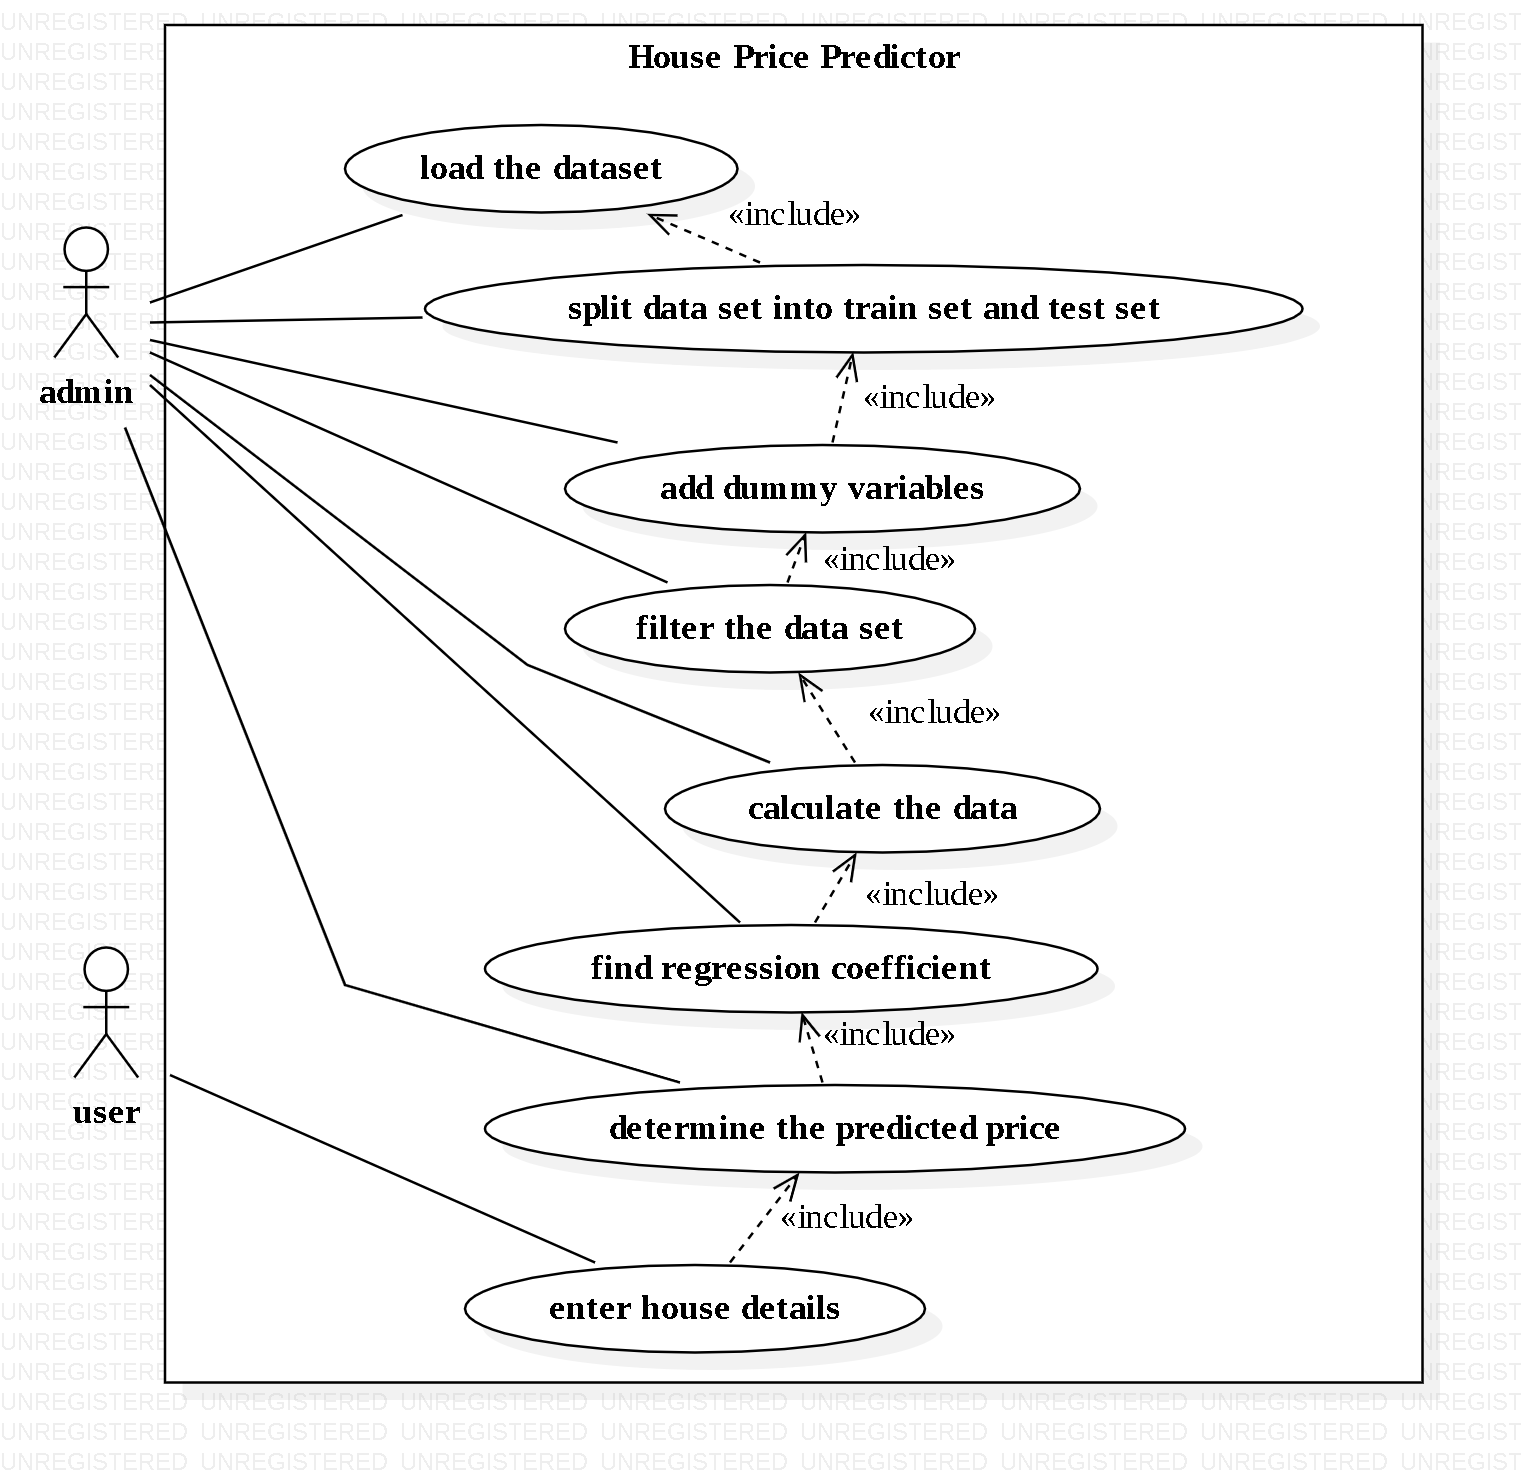
\includegraphics[width=6in]{UseCaseDiagram1.png} 
	\caption{Use case Diagram} %figure name
	%\label{figLaneDetectionusingFeatureSelection} % for referencing
\end{figure}
 \subsection{DFD level diagram}
 %\begin{center}
	%\includegraphics[width = 3in]{images/logo.png}
	%\includegraphics[width = 5in]{images/e.jpg}
	%\caption{Level 0 diagram} %figure name
	%\label{figLaneDetectionusingFeatureSelection} % for referencing
%\end{center}
%\end{figure}\\
A data flow diagram (DFD) maps out the flow of information for any process or system. In Sanskrit OCR system user feeds Data in form of pictures and images to the system to get digitized document as output. \\
%\begin{center}
	%\includegraphics[width = 3in]{images/logo.png}
	%\includegraphics[width = 5in]{images/r.jpg}
	%\caption{Level 1 diagram} %figure name
	%\label{figLaneDetectionusingFeatureSelection} % for referencing
%\end{center}
%\end{figure}\\
\subsection{Software Development Model}
 %\begin{figure}[tbh] % tbh means top, bottom or here (priority: left to right)
%\begin{center}
	%\includegraphics[width = 3in]{images/logo.png}
	%\includegraphics[width = 5in]{images/incre.png}
	%\caption{System Block Diagram} %figure name
	%\label{figLaneDetectionusingFeatureSelection} % for referencing
%\end{center}
%\end{figure}
 Incremental model is a method of software engineering that combines the elements of waterfall model in iterative manner. It involves both development and maintenance. In this model requirements are broken down into multiple modules. Incremental development is done in steps from analysis design, implementation, testing/verification, maintenance. Each iteration passes through the requirements, design, coding and testing phases. The first increment is often a core product where the necessary requirements are addressed, and the extra features are added in the next increments. The core product is delivered to the client. Once the core product is analyzed by the client, there is plan development for the next increment.\\
 Advantages of Incremental Model:
 \begin{itemize}
\item Generates working software quickly and early during the software life cycle.
\item This model is more flexible – less costly to change scope and requirements.
\item It is easier to test and debug during a smaller iteration.
\item In this model customer can respond to each built.
\item Lowers initial delivery cost.
\item Easier to manage risk because risky pieces are identified and handled during it's iteration.

 \end{itemize}
 


\chapter{Epilogue}
\section{Expected Output}
%\begin{figure}[tbh] % tbh means top, bottom or here (priority: left to right)
%\begin{center}
	%\includegraphics[width = 3in]{images/logo.png}
	%\includegraphics[width = 5in]{images/s.jpg}
	%\caption{Expected Output} %figure name
	%\label{figLaneDetectionusingFeatureSelection} % for referencing
%\end{center}
%\end{figure}\\
%\begin{figure}[tbh] % tbh means top, bottom or here (priority: left to right)
%\begin{center}
	%\includegraphics[width = 3in]{images/logo.png}
	%\includegraphics[width = 5in]{images/z.jpg}
	%\caption{Expected Output } %figure name
	%\label{figLaneDetectionusingFeatureSelection} % for referencing
%\end{center}
%\end{figure}
This website will have a good user interface and user experience. In this website, user will have option to either click a picture or upload an image of manuscript/document from camera roll to be digitized. Then this image will go through processes like preprocessing, segmentation, feature extraction, etc. to give the result as shown below. The result can be viewed in the website itself after processing.   

\section{Work Progress and Remaining}
\subsection{Work Completed}
We have read research papers regarding the OCR and the algorithms related to it.\\
•	We collected the datasets required for the project \\
•	We trained datasets for the OCR purpose and also tested the        data for prediction\\
•   We also completed the segmentation algorithm\\
So far, the obtained result is as shown in the figure below
%\begin{center}
	%\includegraphics[width = 3in]{images/logo.png}
	%\includegraphics[width = 5in]{images/x.jpg}
	%\caption{ Output for Testing} %figure name
	%\label{figLaneDetectionusingFeatureSelection} % for referencing
%\end{center}
%\end{figure}

\subsection{Work Remaining}
The following are the remaining works:\\
1.	Integration and post processing\\

%\chapter*{References}
%Reference
\renewcommand\bibname{References} % Change heading to References
\bibliographystyle{IEEEtr} % to use IEEE Format for referencing
\addcontentsline{toc}{chapter}{References} % to add references in TOC
\bibliography{library} % specify the .bib file containing reference information 


\end{document}
